\section{V-n DIAGRAM}

\begin{whitebox}{}
    \begin{tabularx}{\columnwidth}{lclclc}
        $V_A$ & $\unit{m.s^{-1}}$ & Design maneuvering speed\\
        $V_C$ & $\unit{kn}$ & Design cruising speed\\
        $V_D$ & $\unit{kn}$ & Design dive speed\\
        $W$ & $\unit{lbs}$ & Maximum takeoff weight (MTOW)\\
        $\sfrac{W}{S}$ & $\unit{lbs.(ft)^{-2}}$ & Wing loading at design MTOW\\
        $U$ & $\unit{m.s^{-1}}$ & Gust speed\\
        $\sfrac{dc_L}{d\alpha}$ & $\unit{rad^{-1}}$ & Lift slope\\
        $k_g$ & $-$ & Gust alleviation factor\\
        $\mu_g$ & $-$ & Airplane mass ratio\\
        $MAC$ & $\unit{m}$ & Mean aerodynamic chord\\
        $c_{l_\alpha}$ & $\unit{rad^{-1}}$ & Airfoil lift slope\\
        $AR$ & $-$ & Aspect ratio\\
        $b$ & $\unit{m}$ & Wing span
    \end{tabularx}
\end{whitebox}

\begin{highlightbox}{\textbf{CS-23 NORMAL \& COMMUTER CATEGORY}}
    \begin{align*}
        &n_{\max}=2.1+\frac{2400}{W+10000}\\
        &V_C\geq33\sqrt{\frac{W}{S}}\\
        &V_D\geq1.4V_{C,min}
    \end{align*}
\end{highlightbox}

\mathbox{
    &n\overset{\scriptscriptstyle\eqref{eq:lift}, \eqref{eq:stat_turn_load}}{=}\left(\frac{V}{V_{stall}}\right)^2\\
    &V_A=V_{stall}\sqrt{n_{max}}
}

\resizebox{0.9\linewidth}{!}{
    \includegraphics[
    page = {43},
    trim = {1.2cm, 4.5cm, 9.2cm, 4.5cm}, % left, bottom, right, top
    clip
    ]{Lecture04.pdf}
}

\begin{whitebox}{\textbf{GUST ENVELOPE}}
    \begin{whitebox}{NORMALIZED STANDARD GUST}
        \resizebox{1.0\linewidth}{!}{
            \includegraphics[
            page = {44},
            trim = {1.2cm, 12.0cm, 9.5cm, 3.8cm}, % left, bottom, right, top
            clip
            ]{Lecture04.pdf}
        }
    
        \begin{highlightbox}{}
            \begin{align*}
                &\Delta\alpha=\frac{U}{V}\\
                &\Delta L=\frac{1}{2}\rho V^2S_{ref}\frac{dc_L}{d\alpha}\Delta\alpha
            \end{align*}
        \end{highlightbox}
        \blue{Assumptions}
        \begin{itemize}
            \item $L=mg+\Delta L$
        \end{itemize}
        
        \mathbox{
            n=1+\frac{\Delta L}{mg}
        }
    \end{whitebox}

    \begin{highlightbox}{CS-23 CERTIFICATION SPECIFICATION}
        \begin{align*}
            &n=1+k_g\frac{\rho VS_{ref}\frac{dc_L}{d\alpha}U}{2mg}\\
            &k_g=\frac{0.88\mu_g}{5.3+\mu_g}\\
            &\mu_g=\frac{2m}{\rho S_{ref}MAC\frac{dc_L}{d\alpha}}
        \end{align*}
    \end{highlightbox}

    \begin{highlightbox}{WING LIFT SLOPE}
        \begin{align*}
            &\frac{dc_L}{d\alpha}=c_{l_\alpha}\frac{AR}{AR+2}\\
            &AR=\frac{b^2}{S_{ref}}
        \end{align*}
    \end{highlightbox}
    \resizebox{1.0\linewidth}{!}{
        \includegraphics[
        page = {45},
        trim = {1.0cm, 5.0cm, 5.5cm, 2.5cm}, % left, bottom, right, top
        clip
        ]{Lecture04.pdf}
    }

\end{whitebox}

\resizebox{1.0\linewidth}{!}{
    \includegraphics[
    page = {47},
    trim = {3.0cm, 3.5cm, 4.5cm, 4.5cm}, % left, bottom, right, top
    clip
    ]{Lecture04.pdf}
}